
{\emph {We now study modification operations}}. As before, we use bursts of rules and
a similar definition of latency.

\tightparagraph{\bf Table occupancy} To study the impact of table
occupancy, we pre-insert $S$ rules into a switch,
all with the same priority. We then modify one rule at a time by changing the
rule's output port, sending modification requests back to back. 

\begin{figure*}[!tb]
	\centering
        \begin{subfigure}[b]{0.40\textwidth}
                \centering
		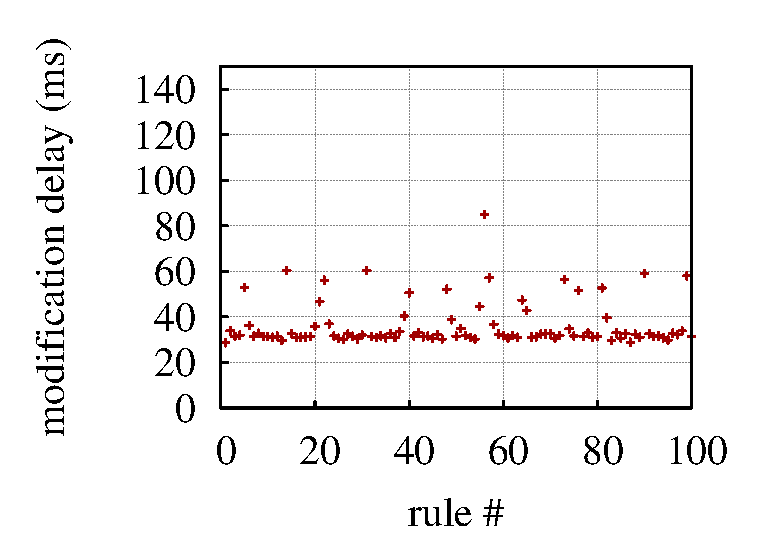
\includegraphics[width=\textwidth]{./figures/mazu/jan27_bcm_mod_same_burst_100_imc.eps}
		\caption{100 rules in table}
		\label{fig:bcm_mod_same_burst_100}
	\end{subfigure}
        \begin{subfigure}[b]{0.40\textwidth}
                \centering
		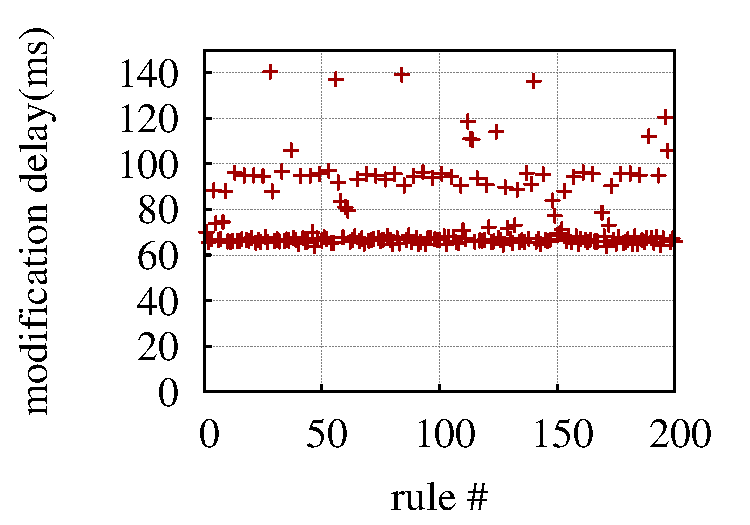
\includegraphics[width=\textwidth]{./figures/mazu/jan27_bcm_mod_same_burst_200-eps-converted-to.pdf}
		\caption{200 rules in table}
		\label{fig:bcm_mod_same_burst_200}
	\end{subfigure}
	\caption{{\bf \BroadcomOne} per-rule {\bf mod.} latency, same priority}
	\label{fig:occupancy-broadcom-modify}
\end{figure*}
 
Per-rule modification delay for \BroadcomOne when $S=100$ and $S=200$ are shown in
\figsref{fig:bcm_mod_same_burst_100}{fig:bcm_mod_same_burst_200}, respectively. We
see that the per-rule delay
is more than 30 ms for $S=100$. When we double the number of rules,
$S=200$, latency doubles as well. It grows
linearly with $S$ (not shown). Note that
this latency is much higher than the corresponding
insertion latency (3.12ms per rule).
\IBM's per-rule modification latency is also affected significantly by the table occupancy---
the per-rule modification latencies for $S=100$ and $S=200$ are 18.77ms and 37.13ms, respectively.
In contrast, \Intel and \BroadcomThree  have lower modification delay,
and it does not vary with table occupancy. For \Intel (\BroadcomThree) the
per-rule modification delay for both $S=100$ and $S=200$ is around 1 ms (2ms)
for all modified rules, similar to (2X more than) same priority insertion delay. 


\tightparagraph{Rule Priority} We conduct two experiments on each switch to
study the impact of rule priority. In
each experiment, we insert $B$ rules into an empty table ($S = 0$). In the 
{\em increasing} priority experiments, the rules in the table each have a
unique priority, and we send back-to-back modification requests for
rules in increasing priority order. We do the opposite in the {\em
decreasing priority} experiment. We vary $B$.%  across

\begin{figure*}[!t]
	\centering
	\begin{subfigure}[b]{0.40\textwidth}
                \centering
		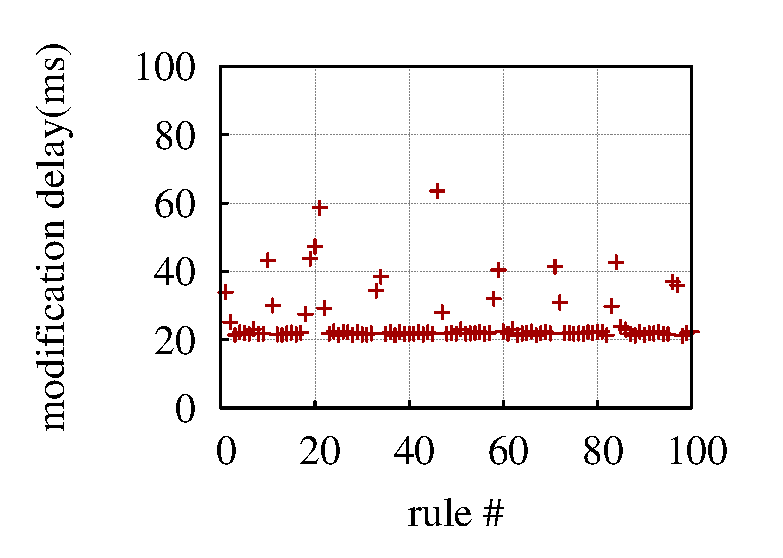
\includegraphics[width=\textwidth]{./figures/mazu/jan27_bcm_mod_incr_burst_100.eps}
		\caption{burst size 100, incr. priority}
		\label{fig:bcm_mod_incr_burst_100}
	\end{subfigure}
        \begin{subfigure}[b]{0.40\textwidth}
                \centering
		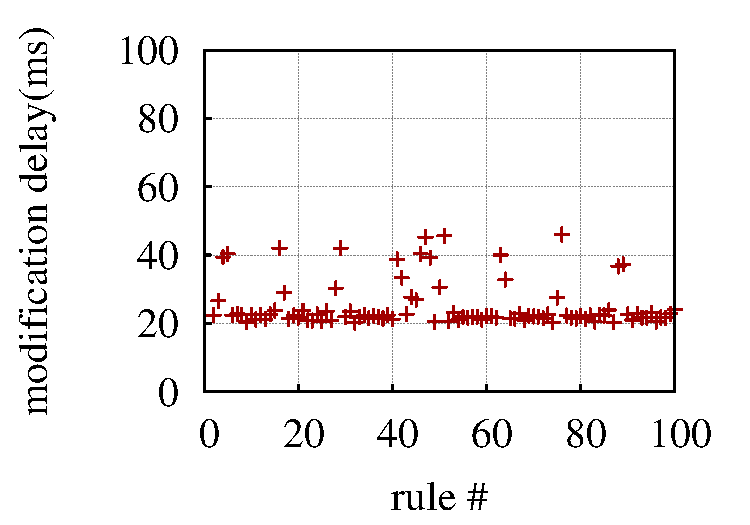
\includegraphics[width=\textwidth]{./figures/mazu/jan27_bcm_mod_decr_burst_100-eps-converted-to.pdf}
		\caption{burst size 100, decr. priority}
		\label{fig:bcm_mod_decr_burst_100}
	\end{subfigure}
	\caption{{\bf \BroadcomOne} priority per-rule {\bf modification} latency}
	\label{fig:priority-broadcom-modify}
\end{figure*}

\figsref{fig:bcm_mod_incr_burst_100}{fig:bcm_mod_decr_burst_100} show the results for the increasing and decreasing priority experiments, respectively, for
$B=100$ on \BroadcomOne. In both cases, we see: (1) the per-rule modification delay is similar
across the rules, with a median of 25.10ms and a standard deviation of
6.74ms, and (2) the latencies are identical across the experiments. 
We similarly observe that priority does not affect modification delay in
\BroadcomThree, \Intel and \IBM (not shown).


\tightparagraph{Summary and root causes}
We conclude that the per-rule modification latency on \BroadcomOne and \IBM is 
impacted purely by table occupancy, not by rule priority structure.
For \BroadcomThree and \Intel, the per-rule modification delay 
is independent of rule priority, table occupancy, and burst size;
\BroadcomThree's per-rule modification delay is 2X higher than insertion.
Conversations with Broadcom indicated that TCAM modification should ideally be fast and independent of table size, 
so the underlying cause appears to be less optimized switch software in \BroadcomOne. Indeed, our measurements with \BroadcomThree show that this issue has (at least partly) been fixed.

